\documentclass{article}

\usepackage[dblblindworkshop]{neurips_2026}
\usepackage[utf8]{inputenc}
\usepackage[T1]{fontenc}
\usepackage{amsmath,amssymb,amsthm}
\usepackage{booktabs}
\usepackage{graphicx}
\usepackage{float}
\usepackage{microtype}
\usepackage{xcolor}
\usepackage{hyperref}
\usepackage{url}
\hypersetup{hidelinks}

\workshoptitle{Representations for the Physical Sciences Workshop}
\title{Noise Covariance as Representation Geometry: One Metric, Four Architecture Classes}
\author{Anonymous Authors}

\newcommand{\R}{\mathbb{R}}
\newcommand{\Sn}{\Sigma}
\newcommand{\Gr}{\mathrm{Gr}}
\newcommand{\range}{\mathrm{range}}
\newtheorem{proposition}{Proposition}
\newtheorem{corollary}{Corollary}

\widowpenalty=10000
\clubpenalty=10000
\begin{document}
\maketitle
\begin{abstract}
Under additive Gaussian noise and constrained low-rank reconstruction, measured observations can supply their own reconstruction supervision: the instrument-characterized noise covariance then determines which residuals are informative. For Gaussian noise, inverse covariance is the likelihood-consistent metric. Rather than proposing a new estimator, we organize classical methods as a pair $(\Sigma^{-1},\mathcal{F})$ that separates measurement geometry from admissible model capacity, and follow one metric across four classes: optimal filtering, unrestricted linear projection, its Kronecker-separable restriction, and factored attention. The linear classes admit an exact geometric characterization. At the Kronecker-separable class, models sharing an architecture but differing only in the training metric reverse their ranking under raw MSE and the likelihood residual, in a frozen ten-seed experiment and a disjoint twenty-seed replication cohort, and under a covariance estimated from $2{,}048$ noise-only events. Each model leading under its own objective is the weaker claim; the substantive result is truth-referenced: the covariance-weighted factors recover the \emph{planted} channel subspace almost exactly and show better exploratory recovery of planted signal parameters, while temporal recovery stays weak. At the attention class the reversal does not appear --- a two-seed pilot favours the covariance-trained arm under \emph{both} metrics, and the benchmark score cannot separate the arms --- so this bounds the claim rather than extending it.
\end{abstract}

\section{Introduction}

Many scientific instruments produce abundant measurements but no labels or clean targets: each observation is its own training signal, and an instrument-derived noise model says which discrepancies matter. Uncertainty varies across frequencies, sensors and conditions; mean-squared error (MSE) weighs all residual coordinates equally, yet under colored noise a large residual can lie in a poorly measured direction while a small one in a low-noise direction is decisive. The measurement covariance is therefore a measurement-model prior fixing the geometry of reconstruction error, distinct from a conservation law or equivariance \citep{bronstein2021geometric,karniadakis2021physics}.

This complements self-supervised reconstruction without clean targets \citep{batson2019noise2self,yaman2020ssdu,gruber2025noisier2inverse}; unlike augmentation- or masking-based self-supervision \citep{chen2020simclr,he2022masked}, which presupposes simulable nuisance structure, measurement noise supplies it directly.

Every individual link is classical; we state the boundary plainly. Inverse-covariance weighting is generalized least squares \citep{aitken1936least} and, at rank one, the matched or optimal filter \citep{turin1960introduction,kay1993fundamentals,szymkowiak1993signal}; that literature fixes the weighting but assumes a \emph{known}, one-dimensional template. The latent-variable line relaxes the signal model but not the noise model: probabilistic PCA assumes isotropic noise \citep{tipping1999probabilistic}, factor analysis a diagonal covariance \citep{rubin1982algorithms,roweis1998algorithms}; weighted low-rank models \citep{bailey2012principal,allen2014gls}, Mahalanobis low-rank representation under two-way correlated noise \citep{zhang2019matrixnormal}, the linear-autoencoder/PCA correspondence \citep{baldi1989neural} and multilinear PCA \citep{lu2008mpca} are all established. \emph{We introduce no new estimator.} What is new is the arrangement: placing these in one $\Sigma^{-1}$ metric as a ladder of admissible representation classes, the exact condition under which the Kronecker restriction is lossless (Proposition~\ref{prop:restricted}), and posing the same metric question to an analogous axis-factored attention network --- so the question does not stop where exact analysis does.

We organize reconstruction methods as a pair $(\Sigma^{-1},\mathcal{F})$: the measurement likelihood fixes the residual geometry $\Sigma^{-1}$, while the architecture fixes the admissible representation class $\mathcal{F}$ --- including the axis along which the data are tokenized (Section~3). Holding $\Sigma^{-1}$ fixed, we walk $\mathcal{F}$ up the four rungs of Section~3: optimal filtering, unrestricted rank-$k$ linear (Proposition~1), Kronecker-separable two-factor (Proposition~2), and factored attention. The first three rungs admit exact geometric characterization (rung 3's joint optimization is nonconvex; its subproblems are exact); the fourth is examined empirically. Nonlinear representation classes beyond attention, distribution shift, and adaptive sampling remain future work.

\section{Covariance-weighted representation geometry}

Let $x_i=s_i+n_i\in\R^d$ be a mean-subtracted observation with $n_i\sim\mathcal{N}(0,\Sigma)$ and $\Sigma\succ0$ (mean handling in Appendix~\ref{app:protocol}). For a candidate reconstruction $\hat{s}_i$, the Gaussian negative log-likelihood is, up to constants,
\begin{equation}
  \chi^2(\hat{s}_i)=(x_i-\hat{s}_i)^\top\Sigma^{-1}(x_i-\hat{s}_i).
  \label{eq:mahalanobis}
\end{equation}
Whitening, $\tilde{x}_i=\Sigma^{-1/2}x_i$, maps this quadratic form to $\|\tilde{x}_i-\hat{\tilde{s}}_i\|_2^2$: the noise-aware problem is Euclidean projection in whitened coordinates and $\Sigma^{-1}$-orthogonal projection in measurement coordinates. We report the mean per-trace residual $N^{-1}\sum_i\chi_i^2$ or the per-coordinate normalized residual $\bar\chi^2=(Nd)^{-1}\sum_{i=1}^{N}\chi^2(\hat{s}_i)$, stating explicitly which normalization is used.

The theory treats $\Sigma$ as specified; in practice it comes from calibration or noise-only records, estimated and regularized without evaluation data, and a misspecified $\Sigma$ defines a misspecified geometry (Appendix~\ref{app:protocol}).

\begin{proposition}[Noise-weighted projection bridge]
\label{prop:bridge}
Under the model above, OF, rank-$k$ covariance-weighted PCA (CW-PCA), and a tied noise-aware linear autoencoder minimize Eq.~\eqref{eq:mahalanobis} over different admissible subspaces. OF fixes a rank-one template; CW-PCA learns a rank-$k$ subspace; and the tied autoencoder parameterizes the same learned projection when its encoder is the $\Sigma^{-1}$-adjoint of its decoder.
\end{proposition}

\paragraph{Proof sketch.}
Whitening reduces the problem to ordinary rank-$k$ approximation, so every minimizer spans a leading eigenspace of the whitened sample covariance; at rank one this is the optimal filter, and the tied $\Sigma^{-1}$-adjoint encoder follows from the same geometry. Unlike the latent-variable precedents of Section~1, the full covariance is kept specified. Details in Appendix~\ref{app:proofs}.

\paragraph{Metric reversal.}
Raw MSE replaces $\Sigma^{-1}$ by $I$ and is likelihood-correct only when $\Sigma=\sigma^2I$; under colored noise MSE follows raw variance while Eq.~\eqref{eq:mahalanobis} emphasizes high-information directions. Consequently, two equal-rank models can satisfy $\mathrm{MSE}(A)<\mathrm{MSE}(B)$ but $\chi^2(A)>\chi^2(B)$, with learned subspaces nearly orthogonal after whitening. This is not an evaluation paradox: each model is optimal in a different geometry.

\section{The architecture ladder}

Holding the metric fixed, we walk the representation class $\mathcal{F}$ of Eq.~\eqref{eq:tuple} up four rungs. Rungs 1--3 are analysed in general two-axis form and evidenced synthetically in Section~4; rung 4 is evidenced on the short-time Fourier transform (STFT) band--frame plane of a public benchmark, where $\Sigma^{-1}$ is diagonal in frequency by measurement (Section~4).

\paragraph{Rung 1: rank-one fixed template (optimal filtering).}
Fixing the signal to a known template $s_0$, the likelihood-optimal reconstruction is the optimal filter (OF) amplitude of Section~2 \citep{gatti1986processing,turin1960introduction}. The representation class is a single direction, and the metric question has a closed-form answer.

\paragraph{Rung 2: unrestricted rank-$k$ linear.}
Replacing the fixed template with a learned rank-$k$ subspace gives covariance-weighted PCA (CW-PCA), which is also the tied noise-aware linear autoencoder: both minimize the likelihood residual over the full Grassmannian $\Gr(k,n_1n_2)$ of a two-axis measurement (Proposition~\ref{prop:bridge}), with reconstruction $\hat s=PP^\top\Sigma^{-1}x$.

\paragraph{Rung 3: Kronecker-separable two-axis projection (NFPA).}
NFPA restricts rung 2's projection to separable factors of a two-axis measurement $Z_i\in\R^{n_1\times n_2}$ --- sensor channel $\times$ time in the controlled synthetic study, frequency band $\times$ time frame on the public benchmark. It learns orthonormal bases $U_1\in\R^{n_1\times k_1}$ and $U_2\in\R^{n_2\times k_2}$, with code $C_i=U_1^\top Z_iU_2$ and reconstruction $\hat Z_i=U_1U_1^\top Z_iU_2U_2^\top$, so that
\begin{equation}
  \mathrm{vec}(\hat Z_i)=\bigl(U_2U_2^\top\otimes U_1U_1^\top\bigr)\mathrm{vec}(Z_i),
  \label{eq:kron-projector}
\end{equation}
and the joint representation is $\range(U_1)\otimes\range(U_2)$. The admissible family is the embedded product
\begin{equation}
  \Gr(k_1,n_1)\times\Gr(k_2,n_2)
  \hookrightarrow \Gr(k_1k_2,n_1n_2).
  \label{eq:product-grassmann}
\end{equation}

\begin{proposition}[Kronecker-restricted bridge]
\label{prop:restricted}
NFPA minimizes the CW-PCA/tied-autoencoder objective restricted to Kronecker-separable two-axis subspaces. Its optimum equals the unrestricted CW-PCA optimum if and only if at least one rank-$k_1k_2$ CW-PCA minimizer has such a separable subspace.
\end{proposition}

\paragraph{Proof sketch.}
Equation~\eqref{eq:kron-projector} is the orthogonal projector onto $\range(U_1)\otimes\range(U_2)$ in whitened coordinates, so NFPA is the whitened rank-$k_1k_2$ objective restricted to Eq.~\eqref{eq:product-grassmann}; equality holds precisely when that set contains an unrestricted minimizer, and otherwise the gap is the cost of the architecture prior, not a failure of the metric. This is a covariance-aware member of the multilinear-PCA family \citep{lu2008mpca}, not a new factorization. When either factor is full rank the restriction is inactive and rung 3 reduces to rung 2; at $k_1=k_2=1$ it recovers rung 1 (Corollary~\ref{cor:rankone}, Appendix~\ref{app:proofs}).

\paragraph{Rung 4: factored attention.}
Rung 3's two-factor restriction, instantiated on the band--frame plane, reads as $\range(U_f)\otimes\range(U_m)$ --- separable frequency-band and time-frame factors; rung 4's transformer performs intra-band temporal attention over frames, then cross-band attention. These are the same factorization at different levels of nonlinearity, in the same coordinates, and $\Sigma^{-1}$ is diagonal in exactly the basis the first factor indexes: on this benchmark a stationary-PSD model fits the readout noise ($\chi^2/\mathrm{dof}=1.0002$, all gates passed; Section~4). The rung-4 model is a transformer \citep{vaswani2017attention} over frame patches \citep{nie2023patchtst}, with rotary embeddings on the temporal axis \citep{su2024roformer} and learned embeddings across bands; the metric question is posed empirically, training identical architecture, data, and budget on two objectives differing only in the metric (Section~4). Injecting the optimal-filter statistic into the forward pass follows prior work on calorimetric event reconstruction \citep{priorThesis} and serves as a secondary contrast.

\section{Evidence}

\begin{figure}[t]
  \centering
  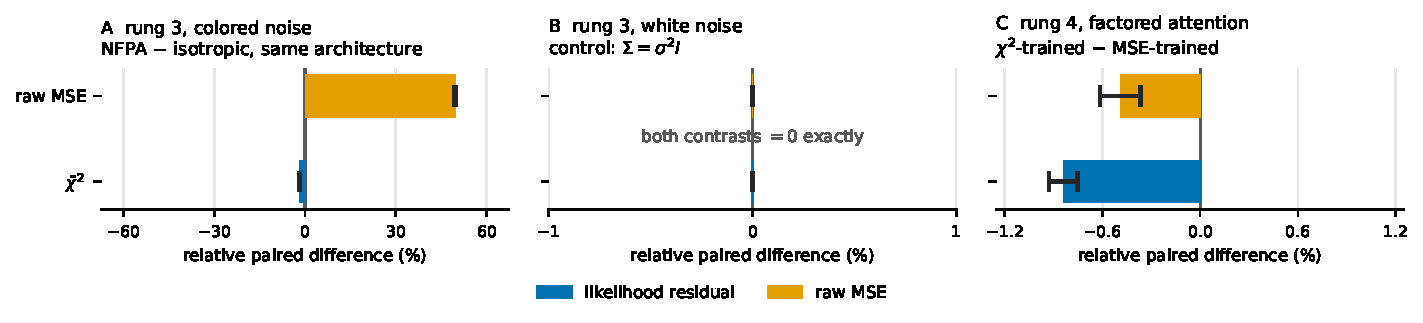
\includegraphics[width=\linewidth]{figures/evidence}
  \caption{\textbf{A}, rung 3: the reversal and its replication. Relative paired
  differences, NFPA minus the isotropic baseline; solid = frozen ten seeds,
  hatched = an independent twenty-seed replication. The metrics point in
  \emph{opposite} directions --- the reversal --- and the cohorts agree.
  Symmetric-log axis (the effects differ by over an order of magnitude);
  cohorts are never pooled. \textbf{B}, what the factors recover at the
  separable condition: the channel subspace almost exactly, the temporal one
  only weakly. Generated from archived summaries.}
  \label{fig:evidence}
\end{figure}

\paragraph{NFPA under channel compression.}
Rung 3 is consolidated at $C=8>k_c=2$ channels, matched rank $k=k_ck_t=6$: NFPA, an isotropically trained factored baseline of the same architecture, CW-PCA, and PCA on the same seeds (superseded rung-2 evidence and the TIDMAD diagnostics motivating the lift are in Appendix~\ref{app:protocol}). NFPA and the isotropic baseline differ only in the training metric, isolating it. It reverses: in the frozen ten-seed experiment NFPA is better under the likelihood residual ($-0.0192$, 95\% interval $[-0.0194,-0.0190]$) and worse under raw MSE ($+0.0034$, $[+0.0034,+0.0034]$), both excluding zero. An independent twenty-seed replication of the identical configuration agrees in sign and magnitude ($-0.0190$, $[-0.0192,-0.0189]$; $+0.0034$, $[+0.0034,+0.0034]$); cohorts are reported separately, any pooled figure being post-hoc rather than a thirty-seed confirmatory experiment. Against unrestricted CW-PCA the residual differs by $-0.0026$ ($[-0.0026,-0.0025]$) --- finite-sample, not evidence the Kronecker restriction is superior. The twenty-seed white-noise run is an identity check: at $\Sigma=\sigma^2I$ the objectives coincide up to scale, and its exact zero shows the pipeline adds no spurious contrast. Estimating the covariance from $2{,}048$ noise-only calibration events preserves the reversal in all ten seeds ($-0.0191$, $[-0.0193,-0.0189]$; $+0.0034$), degrading NFPA's likelihood residual and raw MSE by $0.0078\%$ and $0.0345\%$ of its own oracle held-out values --- consistent with invariance to a global whitening scale and an accurately estimated covariance \emph{shape}, but one fixed condition, not a robustness sweep (Table~\ref{tab:round10}). \looseness=-1

\paragraph{Rung 4 (exploratory): the metric in a factored-attention network.}
One factored-attention architecture is trained on the TIDMAD readout under two objectives differing only in the metric --- \texttt{T-mse} on the unwhitened spectrogram, \texttt{T-chi2} on the $\Sigma^{-1}$-weighted residual --- at matched data, budget and evaluation grid, at two independent seeds. \emph{The reversal does not appear at either seed.} The $\Sigma^{-1}$-trained arm is better on \emph{both} criteria in both runs: held-out paired differences $-1.15$ and $-1.17\times10^{-4}$ on the likelihood residual, $-57.2$ and $-57.4$ on raw MSE, the latter opposite to prediction; all four signs agree across seeds, which bounds run-to-run variation rather than characterising it. The release's coarse score does not separate the arms ($-1.0\times10^{-3}$; window and file-block intervals both span zero), and both arms sit far below the published baselines (Appendix~\ref{app:rung4-baselines}). A degenerate metric would explain it, and we tested for one: $J$ spans a factor $441$ and the whitening weights have coefficient of variation $0.69$, the same order as the rung-3 geometry where the reversal \emph{is} observed ($1.10$; white control $0$). The metric is comparably non-degenerate at both rungs, so the absence is a property of this instantiation, not of the ladder. \looseness=-1

\paragraph{What the covariance-weighted factors recover.}
The metric also changes what the representation \emph{is}. At the separable condition NFPA recovers the planted channel subspace almost exactly ($0.035$ projector error against the isotropic $1.021$) while temporal recovery stays weak ($0.768$ against $1.280$) --- an asymmetry a joint number would hide. All seven paired contrasts --- projector errors and held-out decoding of amplitude, rise time and decay time --- favour NFPA, every seed-level interval excludes zero, and all ten seeds agree in sign. No recovery threshold was predeclared, so these are continuous estimates, not a verdict (Appendix~\ref{app:protocol}).

\paragraph{Transfer of the noise model.}
On a public gravitational-wave strain release \citep{gwoscgw150914,macleod2021gwpy}, a whitened score matching its reference form to $10^{-12}$ and calibrated on synthetic stationary noise (dispersion $1.15$) is seven to nine times over-dispersed on real H1 and L1 strain ($9.42$, $8.83$; leave-one-out $1.77$, $7.29$). A covariance model can be correctly implemented, validated synthetically, and still fail to transfer: implementation identity is not calibration, and transfer is where a learned geometry is falsified.

\paragraph{Limitations.}
The ladder asks whether the likelihood geometry matters and how it interacts with the architecture, in closed form at the linear rungs and empirically at the factored-attention rung, where it is not observed. Five caveats bound the evidence. The rung-4 result is a single seed per arm, so the held-out differences are paired point contrasts over evaluations rather than evidence about seed variability; both arms sit far below the published baselines; and the near-collinearity explanation is inferred from the effect signature, not measured from the whitening spectrum. Rung 4 is one training run per arm, so seed variance is uncharacterized. The linear-rung TIDMAD reversal is not replicated at a confirmatory file. Stationary-PSD adequacy is per-instrument --- adequate on TIDMAD ($\chi^2/\mathrm{dof}=1.0002$), failing on gravitational-wave strain. And the $C=8>k_c=2$ result is synthetic with an oracle covariance, so it bounds what a correctly specified $\Sigma$ buys, not an estimated one.

\paragraph{Takeaway.}
Label-free scientific reconstruction under structured noise should begin with the measurement likelihood rather than treating MSE as a neutral default: $(\Sigma^{-1},\mathcal{F})$ separates the metric from the architecture, the metric question recurs from the optimal filter to factored attention, and its answer is an empirical property of the instrument.


% The neurips_2026 style hides `ack` in the double-blind submission build
% (\let\ack\hide) and typesets it only for camera-ready, which is exactly the
% policy this acknowledgement needs: it names a person, so it must not reach a
% reviewer. Do not convert it into a citation. The rung-4 architecture here is
% our own; the earlier work is an inspiration, not a source model, so a
% citation at the design description would misdescribe the relationship.
\begin{ack}
The idea of posing this reconstruction problem to an axis-factored attention
model was inspired by Sebastian Sjostrom's MSci project on light dark matter
event reconstruction (Imperial College London). No model, code or result of
that work is used here; the architecture, objectives and experiments in this
paper are our own.
\end{ack}

\clearpage
\bibliographystyle{plainnat}
\bibliography{references}

\clearpage
\appendix
\section{Proof details}
\label{app:proofs}

\subsection{Noise-weighted projection bridge}

Let $W=\Sigma^{-1/2}P$. The constraint $P^\top\Sigma^{-1}P=I_k$ becomes $W^\top W=I_k$, and the reconstruction satisfies
\[
 \Sigma^{-1/2}\hat{s}
 =\Sigma^{-1/2}PP^\top\Sigma^{-1}x
 =WW^\top\tilde{x}.
\]
The empirical loss is therefore $N^{-1}\sum_i\|\tilde{x}_i-WW^\top\tilde{x}_i\|_2^2$. By Rayleigh--Ritz, every minimizer spans a leading rank-$k$ eigenspace of the whitened sample covariance. Mapping back yields the CW-PCA subspace. The objective depends on $W$ only through $WW^\top$, so $W$ is identified up to an orthogonal rotation.

\subsection{Whitened signal-plus-identity decomposition}

For $x=s+n$ with $s\perp n$, both zero mean, and $\mathrm{Cov}(n)=\Sigma$: independence gives $\mathrm{Cov}(x)=\mathrm{Cov}(s)+\Sigma$, and conjugating by $\Sigma^{-1/2}$,
\[
 \mathrm{Cov}(\Sigma^{-1/2}x)=\mathrm{Cov}(\Sigma^{-1/2}s)+I.
\]
Adding $I$ shifts every eigenvalue by one and changes no eigenvector, so the eigenvectors of the whitened data covariance are those of the whitened \emph{signal} covariance, in the same order. Rank-$k$ CW-PCA on noisy data therefore recovers the leading whitened signal eigenspace at the population level, which is the precise sense in which the likelihood metric supplies a self-supervised training signal.

\subsection{Kronecker-restricted bridge}

Throughout, the notation is Section~3's: a two-axis measurement $Z\in\R^{n_1\times n_2}$ with factors $U_1\in\R^{n_1\times k_1}$ and $U_2\in\R^{n_2\times k_2}$. Section~4's controlled experiment instantiates the first axis as sensor channel and the second as time, so $(n_1,n_2)=(C,T)$ and $(k_1,k_2)=(k_c,k_t)$ there and in Appendix~\ref{app:protocol}.

\begin{figure}[H]
  \centering
  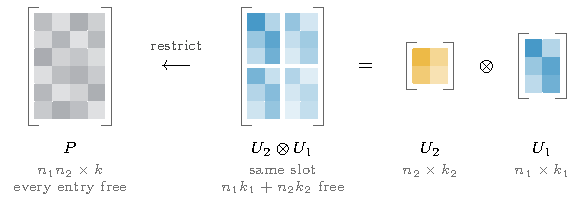
\includegraphics[width=0.78\linewidth]{figures/classes}
  \caption{What the restriction is. Both matrices are a rank-$k$ basis, $k=k_1k_2$,
  for the same vectorised two-axis measurement, so they occupy one slot; on the right the
  entries are not free, the basis being a block grid whose every block is a single
  $U_1$ motif rescaled by one entry of $U_2$. That is why the admissible family is
  the embedded product $\Gr(k_1,n_1)\times\Gr(k_2,n_2)\hookrightarrow
  \Gr(k_1k_2,n_1n_2)$ rather than the full Grassmannian, and why it costs
  $n_1k_1+n_2k_2$ parameters instead of $n_1n_2k_1k_2$. Cell counts show axis
  structure, not Section~4's sizes ($n_1=8$, $n_2=256$, $k_1=2$, $k_2=3$).}
  \label{fig:classes}
\end{figure}


For every such $Z$, the vectorization identity gives
\[
 \mathrm{vec}(U_1U_1^\top ZU_2U_2^\top)
 =(U_2U_2^\top\otimes U_1U_1^\top)\mathrm{vec}(Z).
\]
Column-stacking vectorization puts the \emph{second} axis first, which is why the admissible family is $\range(U_2)\otimes\range(U_1)$ and not the reverse. The Kronecker product is a symmetric idempotent matrix of rank $k_1k_2$, hence the orthogonal projector onto that subspace. NFPA is thus the ordinary whitened rank-$k_1k_2$ projection loss restricted to product subspaces. The restricted and unrestricted minima coincide exactly when an unrestricted minimizing projector belongs to this subset.

\subsection{Rank-one correspondence}

For $Z_i=A_i vt^\top+\epsilon_i$ with isotropic whitened noise and a unique leading signal eigendirection separated by a nonzero eigengap, the population second moment has leading vectorized direction $(t\otimes v)/(\|t\|\|v\|)$, which is feasible for rank-one NFPA. Its projection coefficient is proportional to $\langle \mathrm{vec}(Z_i),t\otimes v\rangle$, the whitened matched-filter coefficient and hence the OF amplitude up to normalization.

\begin{corollary}[Rank-one correspondence]
\label{cor:rankone}
Assume isotropic whitened noise and a unique leading population signal eigendirection separated by a nonzero eigengap. If that direction is generated by a separable template $\tilde{s}=vt^\top$, population NFPA with $k_1=k_2=1$ learns $v/\|v\|$ and $t/\|t\|$ up to signs; its scalar code is proportional to the OF amplitude of Section~2.
\end{corollary}

\section{Experiment details and reporting limits}

The controlled NFPA experiment uses $C=2$ channels, $T=256$ samples, a sampling rate of $1\,\mathrm{kHz}$, channel weights $(1.0,0.65)$, and amplitude $A\sim\mathcal{N}(1,0.3^2)$. The noise is Brownian with $S_n(f)\propto1/f^2$ and is whitened using the matched temporal frequency-domain filter. The train and test sets contain 800 and 300 events. NFPA and IsoAE use $(k_c,k_t)=(2,3)$, while CW-PCA and IsoPCA use rank six.

Because $C=k_c=2$, $U_cU_c^\top=I_2$ in this experiment: the reconstruction restricts a temporal subspace shared by both channels but does not compress the channel axis. Principal angles between NFPA and CW-PCA are $0.0^\circ$, $59.3^\circ$, $64.6^\circ$, $73.8^\circ$, $84.8^\circ$, and $87.8^\circ$ (mean $61.7^\circ$). The corresponding IsoAE--CW-PCA angles are $82.1^\circ$, $83.7^\circ$, $86.0^\circ$, $86.6^\circ$, $88.2^\circ$, and $89.4^\circ$ (mean $86.0^\circ$). These are point estimates from one seed and split, produced by the companion single-split demonstration --- a different experiment and code path from the multi-seed cohorts, and therefore \emph{not} the quantities corrected by E11 (Table~\ref{tab:round10}); the E11 values must not be read as replacements for them. The exact held-out raw-MSE values for IsoAE and IsoPCA are re-exported at full precision from the archived run ($4.58\times10^{-9}$ and $4.33\times10^{-9}$).

\begin{table}[t]
  \centering
  \caption{Implementation check: the single-split $C=k_c=2$ run reported by the earlier draft, retained for provenance. $\bar\chi^2$ is the per-coordinate normalized whitened residual $\bar\chi^2$ of Section~2; $\bar\theta$ is the mean principal angle to CW-PCA in whitened space.}
  \label{tab:results}
  \small
  \setlength{\tabcolsep}{3.8pt}
  \begin{tabular}{lccccc}
    \toprule
    Method & Training & Class & $\bar\chi^2$ & Raw MSE & $\bar\theta$ \\
    \midrule
    CW-PCA & $\Sigma^{-1}$ & full & 0.9929 & $4.95\!\times\!10^{-3}$ & $0^\circ$ \\
    NFPA & $\Sigma^{-1}$ & factored & 0.9916 & $4.95\!\times\!10^{-3}$ & $61.7^\circ$ \\
    IsoAE & MSE & factored & 0.9995 & $4.58\!\times\!10^{-9}$ & $86.0^\circ$ \\
    IsoPCA & MSE & full & 1.0007 & $4.33\!\times\!10^{-9}$ & --- \\
    \bottomrule
  \end{tabular}
\end{table}


\subsection{TIDMAD rung-4 baselines}
\label{app:rung4-baselines}

\begin{table}[t]
  \centering
  \caption{TIDMAD coarse denoising scores (higher is better). \textbf{This
  benchmark's own score cannot separate the two rung-4 arms}, which share
  architecture, data, and budget and differ only in the training objective:
  they return bit-identical values because the upstream aggregation rounds the
  raw score to $0.01$ before the logarithm and both band-limited arms fall in
  the same bin, and rescoring without the rounding gives $0.0241$
  (\texttt{T-mse}) vs.\ $0.0231$ (\texttt{T-chi2}) in band, a contrast whose
  bootstrap interval spans zero (Section~4). Published baselines
  \citep{fry2024tidmad} and the archived linear estimate are full-band and so
  not comparable to the band-limited arms.}
  \label{tab:rung4}
  \small
  \setlength{\tabcolsep}{5pt}
  \begin{tabular}{lc}
    \toprule
    Method & Coarse score \\
    \midrule
    FCNet & 6.55 \\
    Transformer & 4.18 \\
    PUNet & 3.84 \\
    none & 1.10 (1.1026) \\
    linear Wiener (archived) & $-1.8025$ \\
    \texttt{T-mse} & $-2.7708$ \\
    \texttt{T-chi2} & $-2.7708$ \\
    \bottomrule
  \end{tabular}
\end{table}


A submission-strength empirical study should repeat this comparison across seeds and train/test splits and sweep SNR, noise color, channel count, rank pair, and controlled nonseparability. It should report confidence intervals for held-out $\bar\chi^2$, raw MSE, and subspace angles. No such uncertainty estimate is claimed here.

\subsection{Predeclared confirmatory protocol}
\label{app:protocol}
Mean handling, all experiments: the training mean is estimated once, applied unchanged to held-out observations, and added back after reconstruction.

The multi-seed confirmatory study predeclared three hypotheses. \textbf{Executed:} H1 (metric reversal at fixed architecture): under colored or correlated noise, NFPA and an isotropically trained multilinear projection with the same $(k_c,k_t)$ should disagree in ranking, with paired across-seed confidence intervals excluding zero in the predicted directions. H2 (white-noise identity check): when $\Sigma=\sigma^2I$ the two objectives coincide up to scale, so covariance-aware and Euclidean projectors must agree to numerical tolerance; this validates the pipeline rather than the hypothesis. \textbf{Executed later (delayed):} H3 (active restriction): with $C>k_c$ and $T>k_t$, NFPA should recover the planted channel and temporal subspaces for separable signals. This was not run with the original blocks; it was executed afterwards on the archived fits, each of which reproduces its archived held-out residual to $\leq10^{-9}$ relative, so the analysis is computed on the archived fits rather than on refits that merely resemble them. Because the protocol set no numerical recovery threshold, the result is reported as continuous projector errors with seed-level intervals and no binary verdict. Truth-referenced parameter decoding (amplitude, rise time, decay time) was proposed in a block dropped before execution; it is reported at the archived $\alpha=0.1$ condition as \emph{post-hoc exploratory}, and at the separable $\alpha=0$ condition alongside the delayed H3 analysis. An earlier design specified 30 seeds; the executed, frozen protocol is 10 seeds per the 2026-08-08 amendment, fixed before any confirmatory result existed. The primary configuration uses $C=8$ channels, $T=256$ samples, ranks $(k_c,k_t)=(2,3)$, $800/400/2000$ training/validation/test events, $10$ independent seeds, $10$ ALS restarts per seed, SNR $10$ under $\mathrm{SNR}^2=\mathbb{E}[s^\top\Sigma^{-1}s]$, Brownian $1/f^2$ temporal noise with channel correlation, oracle covariance, and nonseparability $\alpha=0.1$. Results enter the main text only if every acceptance gate holds: all seeds complete without post-result configuration changes; the fixed-architecture reversal intervals exclude zero in the predicted directions; the white-noise check passes its predeclared equivalence margin; and the table and figure are generated directly from archived seed-level results.

\paragraph{Rung 3 against the unrestricted rung-2 optimum.} At the frozen $C=8>k_c=2$ configuration the held-out likelihood residual of NFPA differs from unrestricted CW-PCA by $-0.0026$ ($[-0.0026,-0.0025]$). This is a finite-sample difference at matched rank, not evidence that the Kronecker restriction improves on the unrestricted optimum: Proposition~\ref{prop:restricted} gives the only condition under which the restriction is lossless, and it is inactive here.

\paragraph{Semantic recovery, per method.} At the separable condition NFPA attains amplitude RMSE $0.143$ against the isotropic baseline's $0.198$ (decoded-amplitude correlation $0.70$ against $0.13$), and lower rise- and decay-time errors. The same analysis at the archived $\alpha=0.1$ condition is post-hoc exploratory and agrees in direction on all seven contrasts.

The factored representation (Section~3, generic form) has $O(k_1n_1+k_2n_2)$ basis parameters rather than $O(k_1k_2n_1n_2)$ for an unstructured basis, trading approximation flexibility for a two-axis inductive bias related to classical tensor factorizations \citep{kolda2009,lu2008mpca}. Alternating spectral updates solve each factor subproblem exactly, although the joint product-manifold objective remains nonconvex.

\subsection{Round 10: estimated covariance, and the corrected angle diagnostic}
\label{app:round10}

% Generated by scripts/make_rps_round10_table.py -- do not edit by hand.
% Every value is read from an archived summary whose SHA-256 digest is verified
% at build time; see the script for the pinned digests.
\begin{table}[t]
  \centering
  \small
  \caption{Round 10. \textbf{E10b} is a single frozen sensitivity condition:
  the separable covariance is estimated from $2{,}048$ independent noise-only
  calibration events rather than taken as oracle, at the otherwise unchanged
  $C=8>k_c=2$ configuration. The reversal survives in all ten seeds. The
  degradation percentages are relative to NFPA's \emph{own} corresponding
  archived oracle held-out value. This is one condition, not a sweep across
  calibration sizes, covariance families or misspecification.
  \textbf{E11} is a post-hoc diagnostic correction of the whitened-basis
  vectorization used for principal angles; only the \texttt{\_v2} quantities
  carry scientific meaning.}
  \label{tab:round10}
  \begin{tabular}{@{}lr@{}}
    \toprule
    Quantity & Estimate \\
    \midrule
\multicolumn{2}{l}{\emph{E10b --- estimated separable covariance, $N_{\mathrm{cal}}=2048$, 10 seeds}} \\
\quad $\Delta\bar\chi^2$, NFPA $-$ isotropic & $-0.019122$ $[-0.019340,\,-0.018914]$ \\
\quad $\Delta\mathrm{MSE}$, NFPA $-$ isotropic & $+0.0034178$ $[+0.0033963,\,+0.0034393]$ \\
\quad NFPA $\bar\chi^2$ degradation vs.\ oracle & $7.90\times10^{-5}$ (0.0078\%) \\
\quad NFPA MSE degradation vs.\ oracle & $3.55\times10^{-6}$ (0.0345\%) \\
\quad Product-scale ratio vs.\ oracle & $0.9991$ \\
\quad Channel / temporal shape error & $0.0282$ / $0.0197$ \\
\quad Kronecker relative Frobenius error & $0.0365$ \\
\addlinespace
\multicolumn{2}{l}{\emph{E11 --- corrected principal angles to CW-PCA (degrees)}} \\
\quad Frozen, $n=10$ & NFPA $62.89$, isotropic $86.71$, difference $-23.82$ \\
\quad Replication, $n=20$ & NFPA $63.03$, isotropic $86.73$, difference $-23.71$ \\
    \bottomrule
  \end{tabular}
  \par\vspace{2pt}
  \begin{minipage}{\linewidth}\footnotesize
  E11 note: the correction leaves NFPA unchanged and shifts the isotropic
  baseline by $0.81^\circ$ in the frozen cohort and $0.73^\circ$ in the
  replication cohort, so no archived scientific conclusion depended on the
  defect. Intervals are $95\%$ seed-level bootstrap intervals. Cohorts are
  never pooled for confirmatory reading.
  \end{minipage}
\end{table}


E10b repeats the frozen $C=8>k_c=2$ configuration with one change: the separable covariance is estimated from $N_{\mathrm{cal}}=2048$ independent noise-only calibration events instead of being supplied as an oracle. Estimation proceeds by sample estimation of each factor, the regularization already used for the oracle path, and a symmetric product-scale calibration $\hat v=\sqrt{v_cv_t}$ with each factor divided by $\sqrt{\hat v}$; that correction was frozen before any full result existed. The reversal survives in all ten seeds, and the degradation relative to NFPA's own oracle held-out values is small but resolved --- consistent with the fit being invariant to a global whitening scale (the estimated product scale is within $0.1\%$ of oracle) while the covariance \emph{shape} is estimated accurately. This is a single condition: it does not bound behaviour across calibration sizes, covariance families or deliberate misspecification, and no such sweep is claimed.

E11 corrects a vectorization defect in the whitened-basis helper used for principal angles, which unstacked basis columns in the wrong order and so mixed channel and temporal indices. The corrected quantities carry the \texttt{\_v2} suffix. The archival implementation and the legacy columns of the earlier experiments are deliberately left unchanged, so that previously archived tables continue to mean what they meant when written; new analysis uses the corrected path only. The practical consequence of the defect is small: NFPA's mean angle is identical to the legacy value, and the isotropic baseline moves by under one degree in both cohorts, so no archived conclusion depended on it. E11 is a post-hoc diagnostic correction and contributes no confirmatory evidence; in particular it is not a second rung-4 seed --- that role belongs to E7.

\paragraph{Rung-2 numbers carried from the companion work.}
In the 30-seed rank-two benchmark ($512$ traces of dimension $256$ per seed), PCA and CW-PCA had held-out
weighted residuals $48.419$ and $47.869$ (paired difference $0.550$, $[0.530,0.571]$) while raw MSE
preferred the opposite reconstruction, their whitened subspaces $86.25^\circ$ apart. The ten-seed
white-noise control gave a maximum angle of $1.48\times10^{-6}$ degrees. On the TIDMAD file the amplitude
RMSE fell from $0.1209$ to $0.0880$.

\end{document}
